% topic2.tex -- Module 7 Topic 2: Light: wave model, Q19-36.
\topictitle{Topic 2 - Light: Wave Model}

% ---- Q19 (narrower single slit)
\begin{quizq}{}
Monochromatic light passes through a single narrow slit and forms a diffraction pattern on a screen.
The slit is made narrower. What happens to the central bright band?
\opts{It becomes narrower.}{It becomes wider.}{It stays the same width.}{It disappears.}
\end{quizq}

% ---- Q20 (double-slit fringe spacing)
\Needspace{13\baselineskip}
\begin{quizq}{}
Light of wavelength \qty{600}{nm} passes through two slits \qty{0.30}{mm} apart. Bright fringes are seen
on a screen \qty{2.0}{m} away. What is the distance between neighbouring bright fringes?
\opts{\qty{2.0}{mm}}{\qty{4.0}{mm}}{\qty{8.0}{mm}}{\qty{40}{mm}}
\end{quizq}

% ---- Q21 (grating: first-order angle)
\Needspace{12\baselineskip}
\begin{quizq}{}
Light of wavelength \qty{550}{nm} falls on a diffraction grating with 600 lines per millimetre. At what
angle is the first-order maximum?
\opts{\ang{0.33}}{\ang{9.5}}{\ang{19}}{\ang{41}}
\end{quizq}

% ---- Q22 (grating: highest order)
\Needspace{12\baselineskip}
\begin{quizq}{}
For the grating in the previous question (600 lines per millimetre, \qty{550}{nm} light), what is the
highest order of maximum that can be seen?
\opts{1}{2}{3}{4}
\end{quizq}

% ---- Q23 (longer wavelength)
\Needspace{13\baselineskip}
\begin{quizq}{}
In a double-slit experiment, green light is replaced by red light. Everything else stays the same. What
happens to the bright fringes on the screen?
\opts{They move closer together.}{They move further apart.}{They stay in the same places.}
  {They disappear.}
\end{quizq}

% ---- Q24 (one slit covered)
\Needspace{15\baselineskip}
\begin{quizq}{}
In a double-slit experiment, one slit is covered. What pattern is now seen on the screen?
\opts{No light at all reaches the screen.}{The same fringe pattern, but dimmer.}
  {A broad central bright band with much weaker bands on each side, and no closely spaced fringes.}
  {Fringes that are twice as close together.}
\end{quizq}

% ---- Q25 (path difference at a dark fringe)
\Needspace{12\baselineskip}
\begin{quizq}{}
In a double-slit pattern, what is the path difference from the two slits to the SECOND dark fringe from
the centre?
\opts{$\frac{1}{2}\lambda$}{$\lambda$}{$\frac{3}{2}\lambda$}{$2\lambda$}
\end{quizq}

% ---- Q26 (speed of light in water: Newton vs Huygens)
\Needspace{16\baselineskip}
\begin{quizq}{}
In 1850 Foucault showed that light travels more slowly in water than in air. Which model of light did
this support?
\opts{Newton's particle model, because particles are attracted into the water and slow down.}
  {Newton's particle model, because it predicted that light slows down in water.}
  {Neither model, because both predicted that light speeds up in water.}
  {Huygens' wave model, because it predicted that light slows down in a denser medium.}
\end{quizq}

% ---- Q27 (Newton's explanation of refraction)
\Needspace{16\baselineskip}
\begin{quizq}{}
How did Newton's particle model explain the refraction of light as it passes from air into glass?
\opts{The particles are attracted towards the glass surface, so their speed perpendicular to the surface
   increases and they bend towards the normal.}
  {The particles slow down in glass and bend away from the normal.}
  {The wavefronts slow down at the surface, so they change direction.}
  {The particles interfere with each other inside the glass.}
\end{quizq}

% ---- Q28 (two polarisers)
\Needspace{12\baselineskip}
\begin{quizq}{}
Unpolarised light of intensity $I_0$ passes through two polarising filters. The transmission axes of the
filters are at \ang{60} to each other. What is the intensity of the light that comes out?
\opts{$\dfrac{I_0}{2}$}{$\dfrac{I_0}{4}$}{$\dfrac{I_0}{8}$}{$\dfrac{3I_0}{8}$}
\end{quizq}

% ---- Q29 (angle for 75% transmission)
\Needspace{12\baselineskip}
\begin{quizq}{}
Polarised light passes through a polarising filter. At what angle between the light's plane of
polarisation and the filter's axis is 75\% of the intensity transmitted?
\opts{\ang{30}}{\ang{45}}{\ang{60}}{\ang{75}}
\end{quizq}

% ---- Q30 (what polarisation shows)
\Needspace{14\baselineskip}
\begin{quizq}{}
Light can be polarised, but sound cannot. What does this show about light?
\opts{Light travels faster than sound.}{Light is made of particles.}{Light needs no medium.}
  {Light is a transverse wave.}
\end{quizq}

% ---- Q31 (third polariser between crossed polarisers)
\Needspace{14\baselineskip}
\begin{quizq}{}
Two polarising filters are crossed (their axes are at \ang{90}), so no light gets through. A third filter
is placed between them, with its axis at \ang{45} to each of the others. Unpolarised light of intensity
$I_0$ enters the first filter. What intensity comes out of the last filter?
\opts{0}{$\dfrac{I_0}{8}$}{$\dfrac{I_0}{4}$}{$\dfrac{I_0}{2}$}
\end{quizq}

% ---- Q32 (Malus' law graph)
\Needspace{32\baselineskip}
\begin{quizq}{}
Polarised light passes through a polarising filter, which is slowly rotated through \ang{180}. Which graph
shows the transmitted intensity $I$ against the angle $\theta$ between the light's plane of polarisation
and the filter's axis?
\gridopts{%
  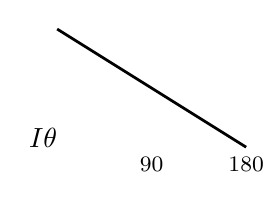
\begin{tikzpicture}\gaxesP{$I$}{$\theta$}
    \draw[line width=1pt] (0,1.5) -- (2.4,0);
    \node[below, font=\footnotesize] at (1.2,0) {\ang{90}}; \node[below, font=\footnotesize] at (2.4,0) {\ang{180}};
  \end{tikzpicture}}
  {%
  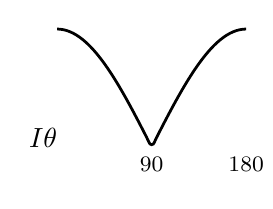
\begin{tikzpicture}\gaxesP{$I$}{$\theta$}
    \draw[line width=1pt, domain=0:2.4, samples=60, smooth] plot (\x, {1.5*abs(cos(75*\x))});
    \node[below, font=\footnotesize] at (1.2,0) {\ang{90}}; \node[below, font=\footnotesize] at (2.4,0) {\ang{180}};
  \end{tikzpicture}}
  {%
  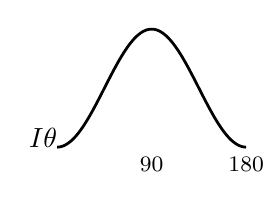
\begin{tikzpicture}\gaxesP{$I$}{$\theta$}
    \draw[line width=1pt, domain=0:2.4, samples=60, smooth] plot (\x, {1.5*(sin(75*\x))^2});
    \node[below, font=\footnotesize] at (1.2,0) {\ang{90}}; \node[below, font=\footnotesize] at (2.4,0) {\ang{180}};
  \end{tikzpicture}}
  {%
  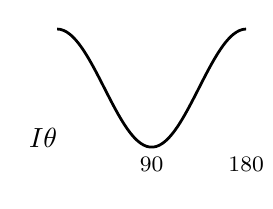
\begin{tikzpicture}\gaxesP{$I$}{$\theta$}
    \draw[line width=1pt, domain=0:2.4, samples=60, smooth] plot (\x, {1.5*(cos(75*\x))^2});
    \node[below, font=\footnotesize] at (1.2,0) {\ang{90}}; \node[below, font=\footnotesize] at (2.4,0) {\ang{180}};
  \end{tikzpicture}}
\end{quizq}

% ---- Q33 (grating compared with a double slit)
\Needspace{15\baselineskip}
\begin{quizq}{}
A double slit is replaced by a diffraction grating with the same slit spacing. How does the pattern
change?
\opts{The bright maxima are at the same angles, but they are much sharper and brighter.}
  {The bright maxima move closer to the centre.}
  {The bright maxima become wider and dimmer.}
  {Only the central maximum remains.}
\end{quizq}

% ---- Q34 (white light through a grating)
\Needspace{16\baselineskip}
\begin{quizq}{}
White light passes through a diffraction grating. Which statement about the pattern is correct?
\opts{The central maximum is red, and violet is furthest from the centre in each spectrum.}
  {The central maximum is violet, and red is closest to the centre in each spectrum.}
  {All colours are diffracted through the same angle, so the pattern is white.}
  {The central maximum is white, and in each spectrum violet is closest to the centre.}
\end{quizq}

% ---- Q35 (diffraction of radio waves and light)
\Needspace{15\baselineskip}
\begin{quizq}{}
A radio can receive a signal behind a large building, but the building casts a sharp shadow in sunlight.
Why?
\opts{Radio waves have long wavelengths, similar to or larger than the building, so they diffract much
   more than light does.}
  {Radio waves travel faster than light.}
  {Light is made of particles, so it cannot diffract.}
  {Radio waves have higher frequencies than light.}
\end{quizq}

% ---- Q36 (CD as a grating)
\Needspace{12\baselineskip}
\begin{quizq}{}
The tracks on a CD are \qty{1.6}{\micro m} apart, so the CD acts as a reflection grating. Red laser light of
wavelength \qty{650}{nm} shines on it. At what angle is the first-order maximum?
\opts{\ang{0.41}}{\ang{24}}{\ang{54}}{\ang{66}}
\end{quizq}
